\documentclass{article}
\usepackage[utf8]{inputenc}

\usepackage{mathtools}
\usepackage{hyperref}
\hypersetup{
    colorlinks=true,
    linkcolor=blue,
    filecolor=magenta,      
    urlcolor=cyan,
}

\title{Brief Summary of Elementary Solutions to Schrödinger's Wave Equation}
\author{Miguel Terán and Andrea Hernandez}
%\date{4 de Mayo de 2020}

\begin{document}

\maketitle

Here we summarize the simple solutions to Schrödinger's wave equation for a variety of solvable potential problems.

\section{FREE PARTICLES $(V=0)$}

\textcolor{blue}{Consider a particle whose potential energy is zero (or has a constant value) at every point in space. The particle is thus not subjected to any force; it is said to be free.}

\textcolor{blue}{When $V(\textbf{x},t)=0$, the Schödinger equation becomes:}
\begin{equation}
    i \hbar \frac{\partial}{\partial t} \psi(\mathbf{x}, t)=-\frac{\hbar^{2}}{2 m} \Delta \psi(\mathbf{x}, t)
    \label{eq1}
\end{equation}


The plane-wave, or momentum, eigenfunction is

\begin{equation}
\psi_{\mathbf{k}}(\mathbf{x}, t)=\frac{1}{(2 \pi)^{3 / 2}} e^{i \mathbf{k} \cdot \mathbf{x}-i \omega t},
\label{eq2}
\end{equation}
where

\begin{equation}
\mathbf{k}=\frac{\mathbf{p}}{\hbar}, \quad \omega=\frac{E}{\hbar}=\frac{\mathbf{p}^{2}}{2 m \hbar}=\frac{\hbar \mathbf{k}^{2}}{2 m},
\label{eq3}
\end{equation}
\\
\textcolor{blue}{and}

\begin{equation}
    E = \frac{\textbf{p}^2}{2m},
\end{equation}
and our normalization is
\begin{equation}
\int \psi_{\mathbf{k}^{\prime}}^{*} \psi_{\mathbf{k}} d^{3} x=\delta^{(3)}\left(\mathbf{k}-\mathbf{k}^{\prime}\right).
\end{equation}
\textcolor{blue}{The density of probability is}
\begin{equation}
    |\psi_{\textbf{k}}(\mathbf{x}, t)|^{2}=|A|^{2}; \qquad A = \frac{1}{(2 \pi)^{3 / 2}}.
\end{equation}
\textcolor{blue}{A plane wave of this type represents a particle whose probability of presence is uniform throughout all space.}
\\

\textcolor{blue}{The principle of superposition tells us that every linear combination of plane satisfying (\ref{eq3}) will also be a solution of equation (\ref{eq1}). Such a superposition can be written: }

\begin{equation}
    \psi(\mathbf{x}, t)=\frac{1}{(2 \pi)^{3 / 2}} \int g(\mathbf{k}) \mathrm{e}^{i[\mathbf{k} \cdot \mathbf{x}-\omega(k) t \mid} \mathrm{d}^{3} k
    \label{eq7}
\end{equation}
\\
\textcolor{blue}{($d^{3}k$ represents, by definition, the infinitesimal volume element in \textbf{k}-space: $dk_x dk_y dk_z$). $g(\textbf{k})$, which can be complex, must be sufficiently regular to allow differentiation inside the integral. It can be shown, morever, that any square-integrable solution can be written in the form (\ref{eq7}). A wave function such as (\ref{eq7}), a superposition of plane waves, is called a three-dimensional "wave packet".} 
\\

The superposition of plane waves leads to the wave-packet description. In the one-dimensional case,
\begin{equation}
    \psi(x, t)=\frac{1}{\sqrt{2 \pi}} \int_{-\infty}^{\infty} d k A(k) e^{i(k x-\omega t)}; \qquad \left(\omega=\frac{\hbar k^{2}}{2 m}\right).
    \label{eq8}
\end{equation}
\textcolor{blue}{In the following paragraph, we shall be intersted in the form of the wave packet at a given instant. If we choose this instant as the time origin, the wave function is written:}
\begin{equation}
    \psi(x, 0)=\frac{1}{\sqrt{2 \pi}} \int dk A(k) \mathrm{e}^{i k x}
    \label{eq9}
\end{equation}
\textcolor{blue}{We see that $A(k)$ is simply the Fourier transform of $\psi(x,0)$:}
\begin{equation}
    A(k)=\frac{1}{\sqrt{2 \pi}} \int dx \psi(x, 0) \mathrm{e}^{-i k x}
\end{equation}
\textcolor{blue}{Consequently, the validity of formula (\ref{eq9}) is not limited to the case of the free particle: whatever the potential, $\psi(x,0)$ can always be written in this form.}
\\

\textcolor{red}{COMMENT: A plane wave of type (\ref{eq2}), whose modulus is constant throughout all space, is not square-integrable. Therefore, rigorosoly, it cannot represent a physical state of a particle. On the other hand, a superposition of plane waves like (\ref{eq8}) can be square-integrable.}
\\

For $|A(k)|$ sharply peaked near $k \simeq k_{0}$, the wave packet moves with a group velocity
\begin{equation}
v_{g} \simeq\left(\frac{d \omega}{d k}\right)_{k_{0}}=\frac{\hbar k_{0}}{m} .
\end{equation}
The time evolution of a minimum wave packet can be described by
\begin{equation}
\psi(x, t)=\left[\frac{(\Delta x)_{0}^{2}}{2 \pi^{3}}\right]^{1 / 4} \int_{-\infty}^{\infty} e^{-(\Delta x)_{0}^{2}\left(k-k_{0}\right)^{2}+i k x-i \omega(k) t} d k, \quad \omega(k)=\frac{\hbar k^{2}}{2 m},
\end{equation}
\\
where
\begin{equation}
\begin{aligned}
|\psi(x, t)|^{2}=&\left\{\frac{1}{2 \pi(\Delta x)_{0}^{2}\left[1+\left(\hbar^{2} t^{2} / 4 m^{2}\right)(\Delta x)_{0}^{-4}\right]}\right\}^{1 / 2} \\
& \times \exp \left\{-\frac{\left(x-\hbar k_{0} t / m\right)^{2}}{2(\Delta x)_{0}^{2}\left[1+\left(\hbar^{2} t^{2} / 4 m^{2}\right)(\Delta x)_{0}^{-4}\right]}\right\}
\end{aligned}
\end{equation}
So the width of the wave packet expands as
\begin{equation}
(\Delta x)_{0} \quad \text { at } t=0 \rightarrow(\Delta x)_{0}\left[1+\frac{\hbar^{2} t^{2}}{4 m^{2}}(\Delta x)_{0}^{-4}\right]^{1 / 2} \quad \text { at } t>0.
\end{equation}

\section{PIECEWISE CONSTANT POTENTIALS IN ONE DIMENSION}

\textcolor{blue}{Shrödinger time-independent equation in one dimension is}

\begin{equation}
    -\frac{\hbar^{2}}{2 m} \frac{d^{2} \psi_{E}(x)}{d x^{2}}+V(x) \psi_{E}(x)=E \psi_{E}(x),
\end{equation}
\\
\textcolor{blue}{where $E$ is the \textit{eigenvalue} of energy and $\psi_{E}(x)$ the \textit{eigenfunction}.}
\\
\\
The basic solutions are
\\
\\
\textcolor{blue}{\textit{Case} $E>V(x)=V_{0}$ :}
\begin{equation}
\begin{aligned}
\frac{d^{2} \psi_E(x)}{d x^{2}}+\underbrace{\frac{2 m}{\hbar^{2}}[E-V_0]}_{k^{2}} \psi_E(x) &=0, \\
\frac{d^{2} \psi_E(x)}{d x^{2}}+k^{2} \psi_E(x) &=0, \\
\frac{d^{2} \psi_E(x)}{d x^{2}} &=-k^{2} \psi_E(x),
\end{aligned}
\end{equation}
\textcolor{blue}{where we have defined,}
\begin{equation}
k^{2}=\frac{2 m}{\hbar^{2}}[E-V_0] \text {. }
\end{equation}
\\
Then, we have the following expressions,
\begin{equation}
E>V=V_{0}: \quad \psi_{E}(x)=c_{+} e^{i k x}+c_{-} e^{-i k x}, \quad k=\sqrt{\frac{2 m\left(E-V_{0}\right)}{\hbar^{2}}}
\end{equation}
\\
\textcolor{blue}{\textit{Case} $E<V(x)=V_{0}$ :}
\begin{equation}
\begin{aligned}
\frac{d^{2} \psi_{E}(x)}{d x^{2}}-\underbrace{\frac{2 m}{h^{2}}\left[V_{0}-E\right]}_{k^{2}} \psi_{E}(x) &=0, \\
\frac{d^{2} \psi_{E}(x)}{d x^{2}}-k^{2} \psi_{E}(x) &=0, \\
\frac{d^{2} \psi_{E}(x)}{d x^{2}}=k^{2} \psi_{E}(x),
\end{aligned}
\end{equation}
where we have defined,
\begin{equation}
k^{2}=\frac{2 m}{h^{2}}\left[V_{0}-E\right].
\end{equation}
\\
Then, we have the following expressions (classically forbidden region):

\begin{equation}
\psi_{E}(x)=c_{+} e^{\kappa x}+c_{-} e^{-\kappa x}, \quad \kappa=\sqrt{\frac{2 m\left(V_{0}-E\right)}{\hbar^{2}}}
\end{equation}
$\left(c_{\pm}\right.$must be set equal to 0 if $x=\pm \infty$ is included in the domain underdiscussion).
\\
\\
\textbf{Rigid-Wall Potential (One-dimensional Box)}
\\
Here (See figure \ref{fig1})
\begin{equation}
V= \begin{cases}0 & \text { for } 0<x<L \\ \infty & \text { otherwise }\end{cases}
\end{equation}
The wave functions and energy eigenstates are

\begin{equation}
\begin{gathered}
\psi_{E}(x)=\sqrt{\frac{2}{L}} \sin \left(\frac{n \pi x}{L}\right), \quad n=1,2,3 \ldots, \\
E=\frac{\hbar^{2} n^{2} \pi^{2}}{2 m L^{2}}
\end{gathered}
\end{equation}
\\
\begin{figure}[h]
    \centering
    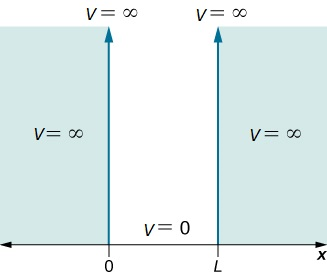
\includegraphics[width=2in]{img1.jpg}
    \caption{The barries outside a one-dimensional box have infinitely large potential, while the interior of the box has a constant, zero potential. } \label{fig1}
\end{figure}
\textbf{Square-Well Potential}
\\
The potential $V$ is (See figure \ref{fig2})
\begin{equation}
V= \begin{cases}0 & \text { for }|x|>a \\ -V_{0} & \text { for }|x|<a \quad\left(V_{0}>0\right).\end{cases}
\end{equation}
The bound-state $(E<0)$ solutions are
\begin{equation}
\psi_{E} \sim \begin{cases}e^{-\kappa|x|} & \text { for }|x|>a, \\
\left.\begin{array}{ll}
\cos k x & \text { (evenparity) } \\
\sin k x & \text { (oddparity) }
\end{array}\right\} & \text { for }|x|<a,\end{cases}
\end{equation}
where
\begin{equation}
k=\sqrt{\frac{2 m\left(-|E|+V_{0}\right)}{\hbar^{2}}}, \quad \kappa=\sqrt{\frac{2 m|E|}{\hbar^{2}}}
\end{equation}
The allowed discrete values of energy $E=-\hbar^{2} \kappa^{2} / 2 m$ are to be determined by solving

\begin{equation}
\begin{array}{ll}
k a \tan k a & =\kappa a \quad  \text { (even parity) } \\
k a \cot k a & =-\kappa a \quad \text { (oddparity). }
\end{array}
\end{equation}
Note also that $\kappa$ and $k$ are related by
\begin{equation}
\frac{2 m V_{0} a^{2}}{\hbar^{2}}=\left(k^{2}+\kappa^{2}\right) a^{2}.
\end{equation}

\begin{figure}[h]
    \centering
    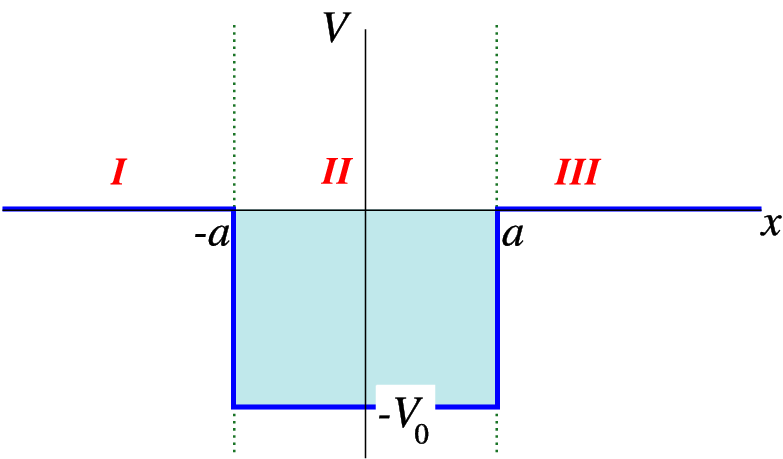
\includegraphics[width=3.0in]{img2.png}
    \caption{The square well potential.} \label{fig2}
\end{figure}
\section{TRANSMISSION-REFLECTION PROBLEMS}

In this discussion we define the transmission coefficient $T$ to be the ratio of the flux of the transmitted wave to that of the incident wave. We consider the following simple examples.
\\
\\
\textbf{Square Well} $\left(V=0\right.$ \textbf{for} $|x|>a, V=-V_{0}$ \textbf{for} $|x|<a$.$)$ (See figure \ref{fig3})
\\
\begin{figure}[h]
    \centering
    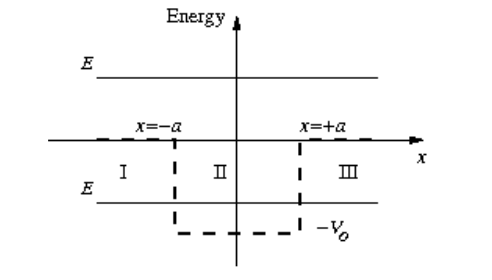
\includegraphics[width=3.0in]{img3.png}
    \caption{The square well potential.} \label{fig3}
\end{figure}

\textcolor{blue}{Let us study the scattering state solutions for $E>0$ in the same way as bound state by considering Schrödinger equations in various regions $I, I I$ and $I I I .$}

\begin{equation}
    \text { Region } I: \quad-\frac{\hbar^{2}}{2 m} \frac{d^{2} \psi_{I}}{d x^{2}}=E \psi_{I} \Rightarrow \frac{d^{2} \psi_{I}}{d x^{2}}+\beta^{2} \psi_{I}=0,
    \label{eq29}
\end{equation}

\begin{equation}
    \text { Region } I I: \quad-\frac{\hbar^{2}}{2 m} \frac{d^{2} \psi_{I I}}{d x^{2}}-V_{0} \psi_{I I}=E \psi_{I I} \Rightarrow \frac{d^{2} \psi_{I I}}{d x^{2}}+k^{2} \psi_{I I}=0,
    \label{eq30}
\end{equation}

\begin{equation}
    \text { Region } I I I: \quad-\frac{\hbar^{2}}{2 m} \frac{d^{2} \psi_{I I I}}{d x^{2}}=E \psi_{I I I} \Rightarrow \frac{d^{2} \psi_{I I I}}{d x^{2}}+\beta^{2} \psi_{I I I}=0,
    \label{eq31}
\end{equation}
\\
\textcolor{blue}{where $\beta^{2}=2 m E / \hbar^{2}$ and $k^{2}=2 m\left(V_{0}+E\right) / \hbar^{2}$. The physically admissible solutions for the above set of Schrödinger equations (\ref{eq29}), (\ref{eq30}) and (\ref{eq31}) are,}

\begin{equation}
    \text { Region } I: \quad \psi_{I}=A e^{i \beta x}+B e^{-i \beta x}
\end{equation}

\begin{equation}
    \text { Region } I I: \quad \psi_{I I}=C \sin (k x)+D \cos (k x)
\end{equation}

\begin{equation}
    \text { Region } I I I: \quad \psi_{I I I}=F e^{i \beta x}+G e^{-i \beta x}
\end{equation}

\textcolor{blue}{If the particle are considered to be moving from left to right with momentum $\beta$, then there is no left-moving particles in region $I I I$ and so we get $G=0$, we have left-moving reflected particles in region $I$ though.}

\textcolor{blue}{The probability current densities of the incident and transmitted particle flux are}

\begin{equation}
    j_{\text {in }}=\frac{\hbar \beta}{m}|A|^{2}; \qquad j_{\mathrm{tr}}=\frac{\hbar \beta}{m}|F|^{2}
\end{equation}

\textcolor{blue}{Therefore the required transmission coefficient is}

\begin{equation}
    T \equiv \frac{j_{\mathrm{tr}}}{j_{\mathrm{in}}}=\frac{|F|^{2}}{|A|^{2}},
\end{equation}
\\
\textcolor{blue}{and the immediate task is to eliminate $B$, $C$ and $D$ using boundary conditions.}
\begin{equation}
\begin{aligned}
T &=\frac{1}{\left\{1+\left[\left(k'^{2}-k^{2}\right)^{2} / 4 k^{2} k^{\prime 2}\right] \sin ^{2} 2 k^{\prime} a\right\}} \\
&=\frac{1}{\left\{1+\left[V_{0}^{2} / 4 E\left(E+V_{0}\right)\right] \sin ^{2}\left(2 a \sqrt{2 m\left(E+V_{0}\right) / \hbar^{2}}\right)\right\}},
\end{aligned}
\end{equation}
where
\begin{equation}
k=\sqrt{\frac{2 m E}{\hbar^{2}}}, \quad k^{\prime}=\sqrt{\frac{2 m\left(E+V_{0}\right)}{\hbar^{2}}}.
\end{equation}
\\
Note that resonances occur whenever
\begin{equation}
2 a \sqrt{\frac{2 m\left(E+V_{0}\right)}{\hbar^{2}}}=n \pi, \quad n=1,2,3, \ldots
\end{equation}
\textbf{Potential Barrier} $\left(V=0\right.$ \textbf{for} $|x|>a, V=V_{0}>0$ \textbf{for} $|x|<a$.$)$ (See figure \ref{fig4})
\begin{figure}[h]
    \centering
    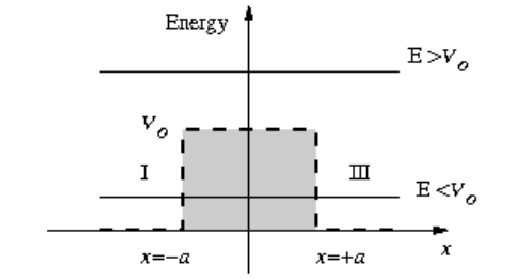
\includegraphics[width=3.0in]{img4.png}
    \caption{The potential barrer.} \label{fig4}
\end{figure}

\\
\textit{Case} $1: E<V_{0}$.
\begin{equation}
\begin{aligned}
T &=\frac{1}{\left\{1+\left[\left(k^{2}+\kappa^{2}\right)^{2} / 4 k^{2} \kappa^{2}\right] \sinh ^{2} 2 \kappa a\right\}} \\
&=\frac{1}{\left\{1+\left[V_{0}^{2} / 4 E\left(V_{0}-E\right)\right] \sinh ^{2}\left(2 a \sqrt{2 m\left(V_{0}-E\right) / \hbar^{2}}\right)\right\}}
\end{aligned}
\end{equation}
\textit{Case} $2: E>V_{0} .$ This case is the same as the square-well case with $V_{0}$ replaced by $-V_{0}$
\\
\\
\textbf{Potential Step} $\left(V=0\right.$ \textbf{for} $x<0, V=V_{0}$ \textbf{for} $x>0$, \textbf{and} $\left.E>V_{0} .\right)$(See figure \ref{fig5})
\begin{figure}[h]
    \centering
    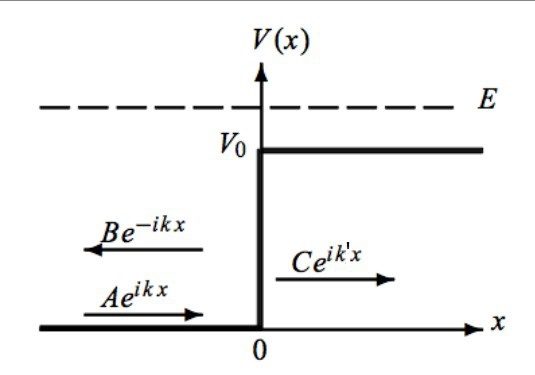
\includegraphics[width=3.0in]{img5.jpg}
    \caption{The potential step.} \label{fig5}
\end{figure}


\begin{equation}
T=\frac{4 k k^{\prime}}{\left(k+k^{\prime}\right)^{2}}=\frac{4 \sqrt{\left(E-V_{0}\right) E}}{\left(\sqrt{E}+\sqrt{E-V_{0}}\right)^{2}}
\end{equation}
with
\begin{equation}
k=\sqrt{\frac{2 m E}{\hbar^{2}}}, \quad k^{\prime}=\sqrt{\frac{2 m\left(E-V_{0}\right)}{\hbar^{2}}}
\end{equation}
\textbf{More General Potential Barrier} $\{V(x)>E$ \textbf{for} $a<x<b, V(x)<E$ \textbf{outside range} $[a, b] .\}$
\\
The approximate JWKB solution for $T$ is
\begin{equation}
T \simeq \exp \left\{-2 \int_{a}^{b} d x \sqrt{\frac{2 m[V(x)-E]}{\hbar^{2}}}\right\}
\end{equation}
where $a$ and $b$ are the classical turning points.${ }^{*}$
\\
\\
\section{SIMPLE HARMONIC OSCILLATOR}

Here the potential is

\begin{equation}
 V(x)=\frac{m \omega^{2} x^{2}}{2},  
\end{equation}

*JWKB stands for Jeffreys-Wentzel-Kramers-Brillouin.
\\

\textcolor{blue}{The Shrödinger time-independent equation with harmonic oscillator potential is}
\begin{equation}
    -\frac{\hbar^{2}}{2 m} \frac{d^{2} \psi_E(x)}{d x^{2}}+\frac{1}{2} m \omega^{2} x^{2} \psi_E(x)=E \psi_E(x)
    \label{eq45}
\end{equation}
\\
\\
and we introduce a dimensionless variable
\begin{equation}
\xi=\sqrt{\frac{m \omega}{\hbar}} x.
\label{eq46}
\end{equation}

\textcolor{blue}{We can write equation (\ref{eq45}) using equation (\ref{eq46}) as}

\begin{equation}
    -\frac{d^{2} \Psi}{d \xi^{2}}+\xi^{2} \Psi=\epsilon \Psi,
    \label{eq47}
\end{equation}
\\
\textcolor{blue}{where}

\begin{equation}
    \epsilon=\frac{2 E}{\hbar \omega}.
\end{equation}

\textcolor{blue}{Case when $\xi \rightarrow \infty$. We can writte equation (\ref{eq47}) as}

\begin{equation}
    \frac{d^{2} \Psi_{\infty}}{d \xi^{2}}-\xi^{2} \Psi_{\infty}=0
    \label{eq49}
\end{equation}
\\
\textcolor{blue}{where $\Psi_{\infty}$ represents the asymptotic solution at infinity. We write the solution of this equation in the form}

\begin{equation}
    \Psi_{\infty}=e^{a \xi^{2}}.
\end{equation}

\textcolor{blue}{We have}

\begin{equation}
    \psi_{\infty}^{\prime \prime}=2 a \psi_{\infty}+4 a^{2} \xi^{2} \psi_{\infty} \approx 4 a^{2} \xi^{2} \psi_{\infty} \quad(\xi \rightarrow \infty).
\end{equation}
\\
\textcolor{blue}{if we put $4a^{2} = 1$ the results coincides with the asymptotic equation; then it must be $a = \pm 1/2$ and we will have as a general asymptotic solution as}

\begin{equation}
    \psi_{\infty}=A e^{\xi^{2} / 2}+B e^{-\xi^{2} / 2}.
    \label{eq52}
\end{equation}

\textcolor{blue}{The physically acceptable solution of ecuation (\ref{eq52}) is}

\begin{equation}
    \psi=e^{-\xi^{2} / 2} u(\xi).
    \label{eq53}
\end{equation}

\textcolor{blue}{Substituting equation (\ref{eq53}) in equation (\ref{eq47}) and simplifying, we obtain the differential equation that determines the function $u(\xi)$}

\begin{equation}
    u^{\prime \prime}-2 \xi u^{\prime}+(\epsilon-1) u=0.
    \label{eq54}
\end{equation}

\textcolor{blue}{It is found that there are polynomial solutions for equation (\ref{eq54}) (and therefore regular) if and only if the parameter $\epsilon - 1$ is an even integer}

\begin{equation}
    \epsilon-1=2 n, \quad n=0,1,2, \ldots
\end{equation}

\textcolor{blue}{In this case the equation reduces to the so-called Hermite equation}

\begin{equation}
    H_{n}^{\prime \prime}-2 \xi H_{n}^{\prime}+2 n H_{n}=0.
\end{equation}
\\
\textcolor{blue}{whose solutions are the Hermite polynomials}

\begin{equation}
    u=H_{n}(\xi)
\end{equation}

\textcolor{blue}{Therefore, the eigenfunctions of the harmonic oscillator are}

\begin{equation}
    \psi_{n}=C_{n} e^{-\xi^{2} / 2} H_{n}(\xi)
\end{equation}
\\
\textcolor{blue}{where $H_{n}$ is the hermittance polynomial of order $n$ and $C_n$ is the normalization constant. Where $C_n$ is} 

\begin{equation}
    C_n = \left(2^{n} n !\right)^{-1 / 2}\left(\frac{m \omega}{\pi \hbar}\right)^{1 / 4}.
\end{equation}

The energy eigenfunctions are
\begin{equation}
\psi_{E}=\left(2^{n} n !\right)^{-1 / 2}\left(\frac{m \omega}{\pi \hbar}\right)^{1 / 4} e^{-\xi^{2} / 2} H_{n}(\xi)
\end{equation}

and the energy levels are
\begin{equation}
E=\hbar \omega\left(n+\frac{1}{2}\right), \quad n=0,1,2, \ldots
\end{equation}
The Hermite polynomials have the following properties:
\begin{equation}
\begin{aligned}
H_{n}(\xi) &=(-1)^{n} e^{\xi^{2}} \frac{\partial^{n}}{\partial \xi^{n}} e^{-\xi^{2}} \\
\int_{-\infty}^{\infty} H_{n^{\prime}}(\xi) H_{n}(\xi) e^{-\xi^{2}} d \xi &=\pi^{1 / 2} 2^{n} ! \delta_{n n^{\prime}} \\
\frac{d^{2}}{d \xi^{2}} H_{n}-2 \xi \frac{d H_{n}}{d \xi}+2 n H_{n} &=0 \\
H_{0}(\xi)=1, \quad H_{1}(\xi) &=2 \xi \\
H_{2}(\xi) &=4 \xi^{2}-2, H_{3}(\xi)=8 \xi^{3}-12 \xi \\
H_{4}(\xi) &=16 \xi^{4}-48 \xi^{2}+12.
\end{aligned}
\end{equation}
\section{THE CENTRAL FORCE PROBLEM [SPHERICALLY SYMMETRICAL POTENTIAL $\boldsymbol{V}=\boldsymbol{V}(\boldsymbol{r})]$}
\\
\\
Here the basic differential equation is

\begin{equation}
\begin{aligned}
-\frac{\hbar^{2}}{2 m}\left[\frac{1}{r^{2}} \frac{\partial}{\partial r}\left(r^{2} \frac{\partial \psi_{E}}{\partial r}\right)\right.\\
&\left.+\frac{1}{r^{2} \sin \theta} \frac{\partial}{\partial \theta}\left(\sin \theta \frac{\partial \psi_{E}}{\partial \theta}\right)+\frac{1}{r^{2} \sin ^{2} \theta} \frac{\partial^{2} \psi_{E}}{\partial \phi^{2}}\right]+V(r) \psi_{E}=E \psi_{E}
\end{aligned}
\end{equation}
where our spherically symmetrical potential $V(r)$ satisfies
\begin{equation}
\lim _{r \rightarrow 0} r^{2} V(r) \rightarrow 0
\end{equation}
The method of separation of variables,
\begin{equation}
\Psi_{E}(\mathbf{x})=R(\tilde{x}) Y_{l}^{m}(\theta, \phi),
\end{equation}
\\
leads to the angular equation
\begin{equation}
-\left[\frac{1}{\sin \theta} \frac{\partial}{\partial \theta}\left(\sin \theta \frac{\partial}{\partial \theta}\right)+\frac{1}{\sin ^{2} \theta} \frac{\partial^{2}}{\partial \phi^{2}}\right] Y_{l}^{m}=l(l+1) Y_{l}^{m},
\end{equation}
where the spherical harmonics
\begin{equation}
Y_{I}^{m}(\theta, \phi), \quad l=0,1,2, \ldots, m=-l,-l+1, \ldots,+l
\end{equation}
satisfy
\begin{equation}
-i \frac{\partial}{\partial \phi} Y_{l}^{m}=m Y_{l}^{m}
\end{equation}
and $Y_{l}^{m}(\theta, \phi)$ have the following properties:

\begin{equation}
\begin{aligned}
Y_{l}^{m}(\theta, \phi) &=(-1)^{m} \sqrt{\frac{2 l}{4 \pi}} \frac{(l-m) !}{(l+m) !} P_{l}^{m}(\cos \theta) e^{i m \phi} \quad \text { for } m \geq 0 \\
Y_{l}^{m}(\theta, \phi) &=(-1)^{|m|} Y_{l}^{|m| *}(\theta, \phi) \quad \text { for } m<0 \\
P_{l}^{m}(\cos \theta) &=\left(1-\cos ^{2} \theta\right)^{m / 2} \frac{d^{m}}{d(\cos \theta)^{m}} P(\cos \theta) \quad \text { for } m \geq 0 \\
P_{l}(\cos \theta) &=\frac{(-1)^{\prime}}{2^{l} l !} \frac{d^{l}\left(1-\cos ^{2} \theta\right)^{l}}{d(\cos \theta)^{\prime}} \\
Y_{0}^{0} &=\frac{1}{\sqrt{4 \pi}}, \quad Y_{1}^{0}=\sqrt{\frac{3}{4 \pi}} \cos \theta \\
Y_{1}^{\pm 1} &=\mp \sqrt{\frac{3}{8 \pi}}(\sin \theta) e^{\pm i \phi} \\
Y_{2}^{0} &=\sqrt{\frac{5}{16 \pi}}\left(3 \cos ^{2} \theta-1\right) \\
Y_{2}^{\pm 1} &=\mp \sqrt{\frac{15}{8 \pi}}(\sin \theta \cos \theta) e^{\pm i \phi} \\
Y_{2}^{\pm 2} &=\sqrt{\frac{15}{32 \pi}}\left(\sin ^{2} \theta\right) e^{\pm 2 i \phi}
\end{aligned}
\end{equation}

\begin{equation}
\int Y_{V^{\prime}}^{m^{\prime *}}(\theta, \phi) Y_{l}^{m}(\theta, \phi) d \Omega=\delta_{I f} \delta_{m m^{\prime}}\left[\int d \Omega=\int_{0}^{2 \pi} d \phi \int_{-1}^{+1} d(\cos \theta)\right]    
\end{equation}


For the radial piece of (A.5.3), let us define
\begin{equation}
u_{E}(r)=r R(r)
\end{equation}

Then the radial equation is reduced to an equivalent one-dimensional problem, namely
\begin{equation}
-\frac{\hbar^{2}}{2 m} \frac{d^{2} u_{E}}{d r^{2}}+\left[V(r)+\frac{l(l+1) \hbar^{2}}{2 m r^{2}}\right] u_{E}=E u_{E}
\end{equation}
subject to the boundary condition
$$
\left.u_{E}(r)\right|_{r=0}=0
$$
For the case of free particles $[V(r)=0$ ] in our spherical coordinates:

\begin{equation}
R(r)=c_{1} j_{l}(\rho)+c_{2} n_{l}(\rho) \quad\left(c_{2}=0 \text { of the origin is included. }\right)
\end{equation}
where $\rho$ is a dimensionless variable
\begin{equation}
\rho \equiv k r, \quad k=\sqrt{\frac{2 m E}{\hbar^{2}}}
\end{equation}
We need to list the commonly used properties of the Bessel functions and sphe\-ri\-cal Bessel and Hankel functions. The spherical Bessel functions are
\begin{equation}
\begin{aligned}
&j l(\rho)=\left(\frac{\pi}{2 \rho}\right)^{1 / 2} J_{l+1 / 2}(\rho) \\
&n_{l}(\rho)=(-1)^{l+1}\left(\frac{\pi}{2 \rho}\right)^{1 / 2} J_{-l-1 / 2}(\rho) \\
&j_{0}(\rho)=\frac{\sin \rho}{\rho}, \quad n_{0}(\rho)=-\frac{\cos \rho}{\rho} \\
&\dot{j}_{1}(\rho)=\frac{\sin \rho}{\rho^{2}}-\frac{\cos \rho}{\rho}, \quad n_{1}(\rho)=-\frac{\cos \rho}{\rho^{2}}-\frac{\sin \rho}{\rho} \\
&j_{2}(\rho)=\left(\frac{3}{\rho^{3}}-\frac{1}{\rho}\right) \sin \rho-\frac{3}{\rho^{2}} \cos \rho \\
&n_{2}(\rho)=-\left(\frac{3}{\rho^{3}}-\frac{1}{\rho}\right) \cos \rho-\frac{3}{\rho^{2}} \sin \rho
\end{aligned}
\end{equation}
For $\rho \rightarrow 0$, the leading terms are
\begin{equation}
j_l(\rho) \underset{\rho \rightarrow 0}{\longrightarrow} \frac{\rho^{l}}{(2 l+1) ! !}, \quad n_{l}(\rho) \underset{\rho \rightarrow 0}{\longrightarrow}-\frac{(2 l-1) ! !}{\rho^{l+1}}
\end{equation}
where
\begin{equation}
(2 l+1) ! !=(2 l+1)(2 l-1) \cdots \cdot 5 \cdot 3 \cdot 1
\end{equation}
\\
In the large $\rho$-asymptotic limit, we have
\begin{equation}
\begin{aligned}
&j_{l}(\rho) \underset{\rho \rightarrow \infty}{\longrightarrow} \frac{1}{\rho} \cos \left[\rho-\frac{(l+1) \pi}{2}\right], \\
&n_{l}(\rho) \underset{\rho-\infty}{\longrightarrow} \frac{1}{\rho} \sin \left[\rho-\frac{(l+1) \pi}{2}\right] .
\end{aligned}
\end{equation}
Because of constraints (A.5.8) and (A.5.9), $R(r)$ must be finite at $r=0$; hence, from (A.5.10) and (A.5.13) we see that the $n_{l}(\rho)$-term must be deleted because of its singular behavior as $\rho \rightarrow 0$. Thus $R(r)=c_{l} j_{l}(\rho)$ [or, in the notation of Chapter 6 , Section $\left.6.4, A_{l}(r)=R(r)=c_{l} j_{l}(\rho)\right]$. For a three-dimensional squarewell potential, $V=-V_{0}$ for $r<R$ (with $V_{0}>0$ ), the desired solution is
\begin{equation}
R(r)=A_{l}(r)=\text { constant } j_{l}(\alpha r)
\end{equation}
where
\begin{equation}
\alpha=\left[\frac{2 m\left(V_{0}-|E|\right)}{\hbar^{2}}\right]^{1 / 2}, \quad r<R
\end{equation}
As discussed in $(7.6 .30)$, the exterior solution for $r>R$, where $V=0$, can be written as a linear combination of spherical Hankel functions. These are defined as follows:
\begin{equation}
\begin{aligned}
h_{l}^{(1)}(\rho) &=j_{l}(\rho)+i n_{l}(\rho) \\
h_{l}^{(1) *}(\rho) &=h_{l}^{(2)}(\rho)=j_{l}(\rho)-i n_{l}(\rho)
\end{aligned}
\end{equation}
which, from (A.5.15), have the asymptotic forms for $\rho=\infty$ as follows:
\begin{equation}
\begin{gathered}
h_{l}^{(1)}(\rho) \underset{\rho \rightarrow \infty}{\longrightarrow} \frac{1}{\rho} e^{i[\rho-(l+1) \pi / 2 \mid} \\
h_{l}^{(1) *}(\rho)=h_{l}^{(2)}(\rho) \underset{\rho \rightarrow \infty}{\longrightarrow} \frac{1}{\rho} e^{-i[\rho-(l+1) \pi / 2]}
\end{gathered}
\end{equation}
If we are interested in the bound-state energy levels of the three-dimensional square-well potential, where $V(r)=0, r>R$, we have
\begin{equation}
\begin{aligned}
u_{j}(r) &=r A_{l}(r)=\text { constant } e^{-\kappa r} f\left(\frac{1}{x r}\right) \\
\kappa &=\left(\frac{2 m|E|}{\hbar^{2}}\right)^{1 / 2}
\end{aligned}
\end{equation}
To the extent that the asymptotic expansions, of which (A.5.19) give the leading terms, do not contain terms with exponent of opposite sign to that given, we have-for $r>R$ - the desired solution from $(\mathrm{A} .5 .20)$ :
\begin{equation}
A_{l}(r)=\operatorname{constant} h_{l}^{(1)}(i \kappa r)=\operatorname{constant}\left[j_{l}(i k r)+i n_{i}(i \kappa r)\right]
\end{equation}

where the first three of these functions are
\begin{equation}
\begin{aligned}
h_{0}^{(1)}\left(i_{k r}\right) &=-\frac{1}{\kappa r} e^{-\kappa r} \\
h_{1}^{(1)}(i \kappa r) &=i\left(\frac{1}{k r}+\frac{1}{\kappa^{2} r^{2}}\right) e^{-\kappa r} \\
h_{2}^{(1)}(i \kappa r) &=\left(\frac{1}{k r}+\frac{3}{\kappa^{2} r^{2}}+\frac{3}{\kappa^{3} r^{3}}\right) e^{-\kappa r}
\end{aligned}
\end{equation}
Finally, we note that in considering the shift from free particles $[V(r)=0]$ to the case of the constant potential $V(r)=V_{0}$, we need only replace the $E$ in the free-particle solution [see (A.5.10) and (A.5.11) by $E-V_{0}$. Note, however, that if $E<V_{0}$, then $h_{l}^{(1,2)}(i \kappa r)$ is to be used with $\kappa=\sqrt{2 m\left(V_{0}-E\right) / \hbar^{2}}$

\section{HYDROGEN ATOM}

%o tambien puedes seleccionar toda una pagina y la convierte en latex, asi pase en apendice de napolitano a latex
%que inteligente hehe bueno dejame leer y buscarle como ir haciendolo
%ok
%lo que vayas agregando ponlo en otro color para que el profe vea que es un agrgado y no parte del napolitano.. lo haces con %\textcolor{blue}{Aquí va el texto} .. puedes usar otro color si gustas
\textcolor{blue}{The hydrogen atom is a system formed by two particles, a nucleus of mass $\mathrm{m}_{\mathrm{N}} $
and charge $+\mathrm{Ze}$, where $\mathrm{Z}=1$, is the nuclear charge, and an electron of mass $\mathrm{m}_{\mathrm{e}}$ and charge $-\mathrm{e}$.}


\textcolor{blue}{The system must include the kinetic energies of both particles, as well as the potential energy of interaction between them, given by Coulomb's law.}

\begin{equation}
    \mathrm{H}=\mathrm{T}+\mathrm{V}=-\frac{\hbar^{2}}{2 \mathrm{~m}_{\mathrm{N}}} \nabla_{\mathrm{N}}^{2}-\frac{\hbar^{2}}{2 \mathrm{~m}_{\mathrm{e}}} \nabla_{\mathrm{c}}^{2}-\frac{\mathrm{Ze}^{2}}{\mathrm{r}}
\end{equation}

Here the potential is

\begin{equation}
V(r)=-\frac{Z e^{2}}{r}
\end{equation}
and we introduce the dimensionless variable
\begin{equation}
\rho=\left(\frac{8 m_{e}|E|}{h^{2}}\right)^{1 / 2} r.
\end{equation}

\textcolor{blue}{The problem of the hydrogen atom is a problem of central forces so it is possible to write the complete Hamiltonian through the relation:}

 \begin{equation}
     \mathrm{H}=\mathrm{T}+\mathrm{V}=-\frac{\hbar^{2}}{2 \mathrm{M}} \nabla_{\mathrm{R}}^{2}-\frac{\hbar^{2}}{2 \mu} \nabla_{\mathrm{r}}^{2}-\frac{\mathrm{Ze}^{2}}{\mathrm{r}}=\mathrm{H}_{\mathrm{R}}+\mathrm{H}_{\mathrm{r}}
 \end{equation}
 
 \textcolor{blue}{Thus, in spherical polar coordinates,}
 \begin{equation}
   \mathrm{H}(r, \theta, \phi) \psi(r, \theta, \phi)=E \psi(r, \theta, \phi)\\
\end{equation}
 \textcolor{blue}{becomes}
 \begin{equation}
\begin{array}{r}
{\left[\frac{-h^{2}}{2 \mu}\left(\frac{1}{r^{2}} \frac{\partial}{\partial r}\left(r^{2} \frac{\partial}{\partial r}\right)+\frac{1}{r^{2} \sin \theta} \frac{\partial}{\partial \theta}\left(\sin \theta \frac{\partial}{\partial \theta}\right)+\frac{1}{r^{2} \sin ^{2} \theta} \frac{\partial^{2}}{\partial \phi^{2}}\right)+V(r, \theta, \phi)\right]} \\
\times\psi(r, \theta, \phi)=E \psi(r, \theta, \phi)
\end{array}
\end{equation}
 \textcolor{blue}{recall}
 \begin{equation}
    \hat{L}^{2}=-\hbar^{2}\left(\frac{1}{r^{2} \sin \theta} \frac{\partial}{\partial \theta}\left(\sin \theta \frac{\partial}{\partial \theta}\right)+\frac{1}{r^{2} \sin \theta} \frac{\partial^{2}}{\partial \phi^{2}}\right)
\end{equation}
 
 \textcolor{blue}{Thus, we can rewrite the Schrodinger equation as:}
 \begin{equation}
    \left[-\hbar^{2}\left(\frac{\partial}{\partial r}\left(r^{2} \frac{\partial}{\partial r}\right)\right)+2 \mu r^{2}[V(r)-E]\right] \psi(r, \theta, \phi)+\hat{L}^{2} \psi(r, \theta, \phi)=0
\end{equation}

\textcolor{blue}{Recalling that the spherical
harmonics are eigenfunctions of the angular momentum operator:}
\begin{equation}
    \psi(r, \theta, \phi)=R(r) Y_{l}^{m}(\theta, \phi) \quad \text { Separation of Variables }
\end{equation}
 \textcolor{blue}{The equation for the radial function is given by}
 \begin{equation}
    \left[-\frac{\hbar^{2}}{2 \mu r^{2}} \frac{d}{d r}\left(r^{2} \frac{d R}{d r}\right)+\frac{l(l+1) \hbar^{2}}{2 \mu r^{2}}+V(r)\right] R=E R
\end{equation}
\textcolor{blue}{to make the equation dimensionless, we define a new variable}
\begin{equation}
    \rho=\alpha r
\end{equation}
\textcolor{blue}{doing a bit of algebra we can write the above equation as follows}
\begin{equation}
    \frac{1}{\rho^{2}} \frac{d}{d_{\rho}}\left(\rho^{2} \frac{d R}{d \rho}\right)+\left(\frac{\lambda}{\rho}-\frac{1}{4}-\frac{l(l+1)}{\rho^{2}}\right) R=0
\end{equation}
\textcolor{blue}{where}
\begin{equation}
    \alpha^{2}=\frac{8 \mu|E|}{\hbar^{2}} 
\end{equation}
\textcolor{blue}{and}
\begin{equation}
     \lambda=\frac{2 \mu Z e^{2}}{\alpha h^{2}}=\frac{Z e^{2}}{\hbar}\left(\frac{\mu}{2|E|}\right)^{\frac{1}{2}}
\end{equation}
\textcolor{blue}{Using the asymptotic method we deduce}
\begin{equation}
    \rho^{2} L^{\prime \prime}+\rho[2(s+1)-\rho] L^{\prime}+[\rho(\lambda-s-1)+s(s+1)-l(l+1)] L=0
\end{equation}
\textcolor{blue}{If $\rho$ is set equal to zero in this equation, it follows from the form of $L$ that $s(s+1)-l(l+1)=0 .$ This quadratic equation in $s$ has two roots: $s=l$ and $s=-(l+1)$. The boundary condition that $R(\rho)$ be finite at $\rho=0$ requires that we choose $s=l$. The equation for $I$, then becomes}

\begin{equation}
    \rho L^{\prime \prime}+[2(l+1)-\rho] L^{\prime}+(\lambda-l-1) L=0
\end{equation}
\textcolor{blue}{The recursion relalion between the coefficients of suecessive lerms of the series is reulily seen to be}
\begin{equation}
    a_{v+1}=\frac{\nu+l+1-\lambda}{(\nu+1)(\nu+2 l+2)} a_{\nu}
\end{equation}

\textcolor{blue}{The radial wave function is of the form $e^{-\frac{i}{3} \rho} \rho^{l} L_{n+1}^{2 l+1}(\rho)$. The normalization constant may be found by using the generating function to evaluate the integral}
\begin{equation}
    \int_{0}^{\infty} c^{-\rho} \rho^{2 l}\left[L_{n+l}^{2 l+1}(\rho)\right]^{2} \rho^{2} d \rho=\frac{2 n[(n+l)]]^{3}}{(n-l-1) !}
\end{equation}

\textcolor{blue}{Finally the Radial eigenfunctions are}
\begin{equation}
    R_{n l}(r)=-\left[\frac{(n-l-1) !}{2 n[(n+l) !]^{3}}\right]^{\frac{1}{2}}\left(\frac{2 Z}{n a_{o}}\right)^{l+\frac{3}{2}} r^{l} e^{\frac{-Z_{r}}{n a_{o}}} L_{n+l}^{2 l+1}\left(\frac{2 Z r}{n a_{o}}\right)
\end{equation}
 \textcolor{blue}{with}
 \begin{equation}
     a_{o}=\frac{\epsilon_{o}^{2} h^{2}}{\pi \mu e^{2}}
 \end{equation}
 
The energy eigenfunctions and eigenvalues (energy levels) are
\begin{equation}
\begin{aligned}
\psi_{n l m} &=R_{n l}(r) Y_{l}^{m}(\theta, \phi) \\
 \\
E_{n} &\left.=\frac{-Z^{2} e^{2}}{2 n^{2} a_{0}} \quad \text { (independent of } l \text { and } m) \\
a_{0} &=\text { Bohr radius } \\
&n \geq l+1, \quad \rho=\frac{2 Z r}{m a_{0}}.
\end{aligned}
\end{equation}
The associated Laguerre polynomials are defined asfollows:
\begin{equation}
L_{p}^{q}(\rho)=\frac{d^{q}}{d \rho^{q}} L_{p}(\rho)
\end{equation}
\\
where-in particular-
\begin{equation}
L_{p}(\rho)=e^{\rho} \frac{d^{p}}{d \rho^{p}}\left(\rho^{p} e^{-p}\right)
\end{equation}
and the normalization integral satisfies
\begin{equation}
\int e^{-\rho} \rho^{2 l}\left[L_{n+l}^{2 l+1}(\rho)\right]^{2} \rho^{2} d \rho=\frac{2 n[(n+l) !]^{3}}{(n-l-1) !} .
\end{equation}
The radial functions for low $n$ are
\begin{equation}
\begin{aligned}
&R_{10}(r)=\left(\frac{Z}{a_{0}}\right)^{3 / 2} 2 e^{-2 r / a_{0}} \\
&R_{20}(r)=\left(\frac{Z}{2 a_{0}}\right)^{3 / 2}\left(2-Z r / a_{0}\right) e^{-2 r / 2 a_{0}} \\
&R_{21}(r)=\left(\frac{Z}{2 a_{0}}\right)^{3 / 2} \frac{Z r}{\sqrt{3} a_{0}} e^{-2 r / 2 \omega_{0}}
\end{aligned}
\end{equation}
The radial integrals are
\begin{equation}
\begin{aligned}
\left\langle r^{k}\right\rangle & \equiv \int_{0}^{\infty} d r r^{2+k}\left[R_{n l}(r)\right]^{2} \\
\langle r\rangle &=\left(\frac{a_{0}}{2 Z}\right)\left[3 n^{2}-l(l+1)\right] \\
\left(r^{2}\right\rangle &=\left(\frac{a_{0}^{2} n^{2}}{2 Z^{2}}\right)\left[5 n^{2}+1-3 l(l+1)\right] \\
\left\langle\frac{1}{r}\right) &=\frac{Z}{n^{2} a_{0}} \\
\left\langle\frac{1}{r^{2}}\right\rangle &=\frac{Z^{2}}{\left[n^{3} a_{0}^{2}\left(l+\frac{1}{2}\right)\right]}
\end{aligned}
\end{equation}

\end{document}

